\section{Introduction}%
\frame{\tableofcontents[currentsection]}

\begin{frame}{Clinical Trial Design has Many Gatekeepers}
\begin{figure}
    \centering
    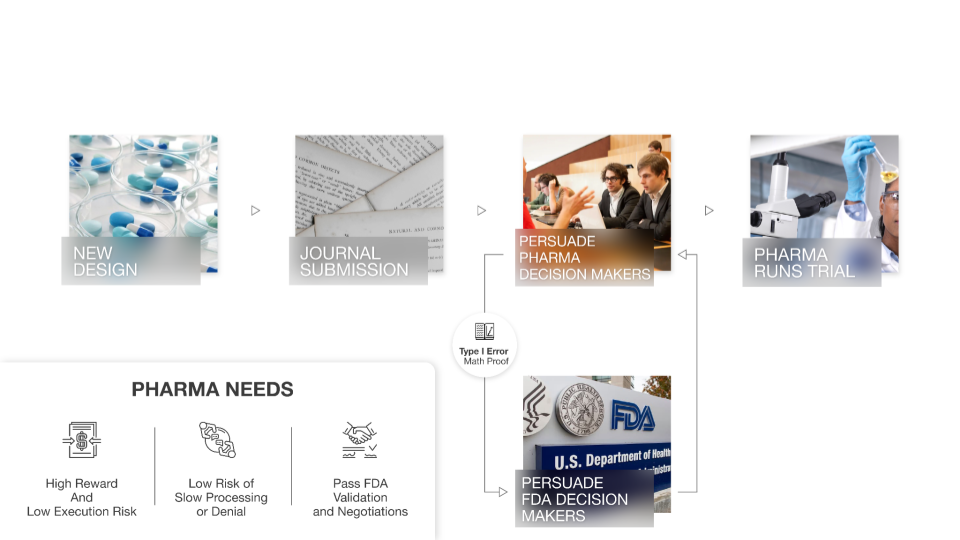
\includegraphics[width=\linewidth]{figs/motivation-3.png}
\end{figure}
\end{frame}

\begin{frame}{Our Goal: Automate Analysis of Simulations}
\begin{figure}
    \centering
    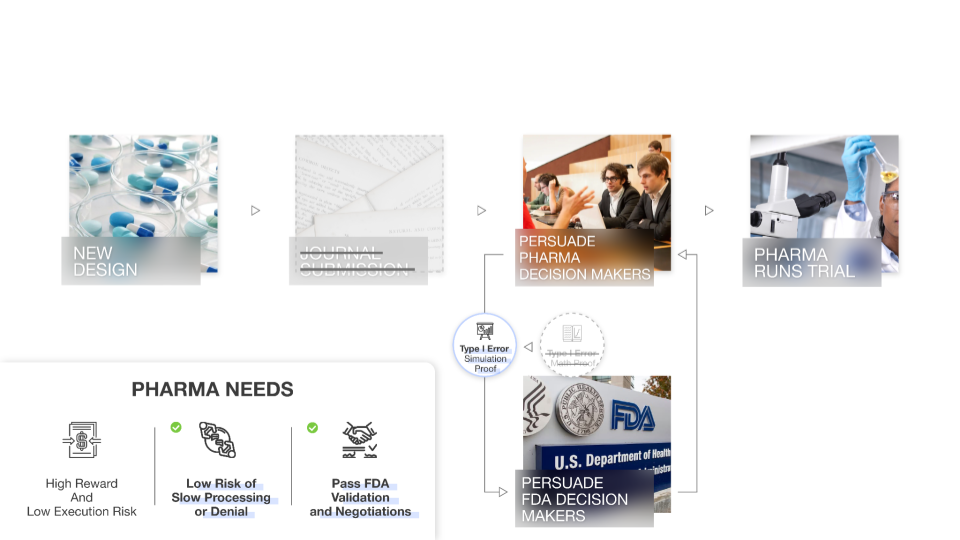
\includegraphics[width=\linewidth]{figs/motivation-4.png}
\end{figure}
\end{frame}

\begin{frame}{Our Goals: Recap}
\begin{itemize}
    \item Predictable and fast trial design innovation!
    \item Automate design validation.
    \item Rigorous analysis for complex designs.
\end{itemize} 
\end{frame}

\begin{frame}{Simulation Raises New Challenges}
\begin{itemize}
    \item Simulation constrained to \textbf{finite} number of null points.
    \begin{center}
        \textbf{How do we deal with composite nulls?}
    \end{center}
    \item Simulation has Monte Carlo error. 
    \begin{center}
        \textbf{How do we deal with Monte Carlo error?}
    \end{center}
    \item Bounded computing power.
    \begin{center}
        \textbf{How many points in the null space to simulate?}
    \end{center}
    \begin{center}
        \textbf{Are the simulations even tractable?}
    \end{center}
\end{itemize}
\end{frame}

\begin{frame}{Intuition for Composite Null}
\begin{figure}
    \centering
    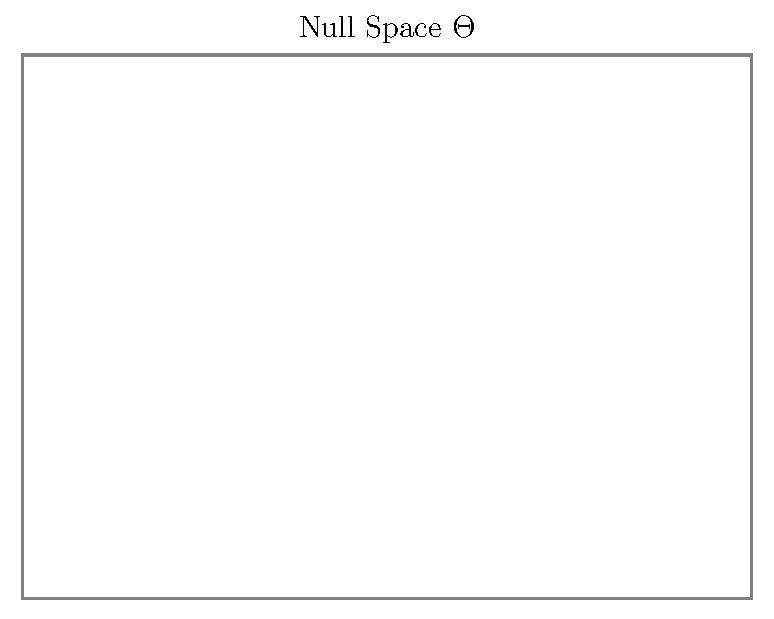
\includegraphics[width=0.95\linewidth]{figs/approach_1.pdf}
\end{figure} 
\end{frame}

\begin{frame}{Partition $\Theta$ into Tiles with Representatives}
\begin{figure}
    \centering
    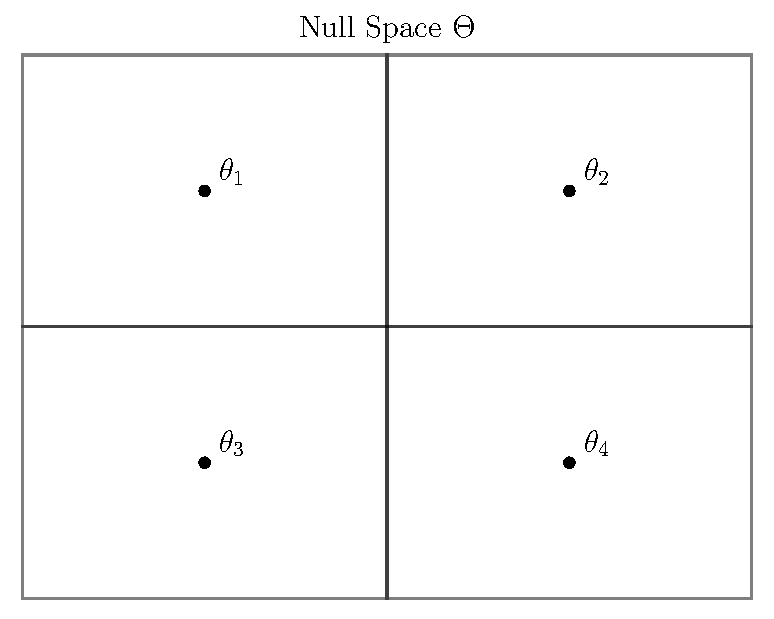
\includegraphics[width=0.95\linewidth]{figs/approach_2.pdf}
\end{figure} 
\end{frame}

\begin{frame}{Simulate on each Representative}
\begin{figure}
    \centering
    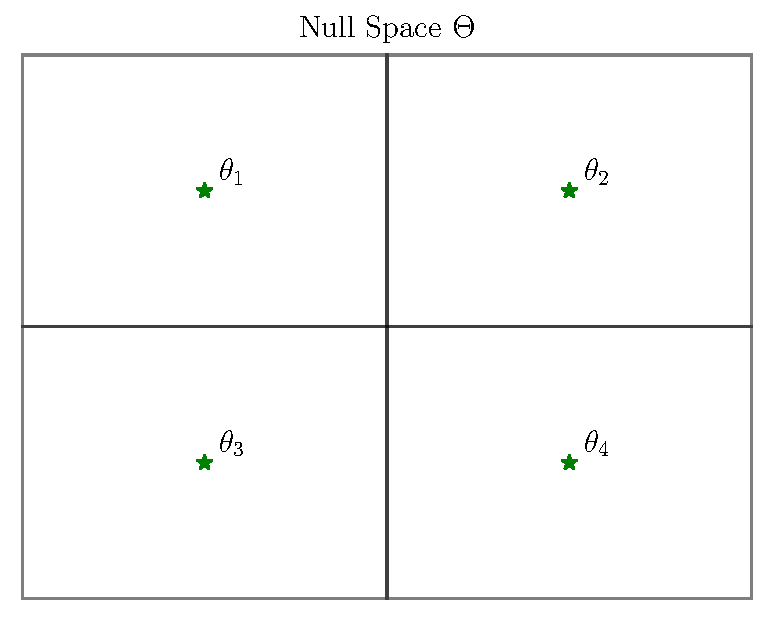
\includegraphics[width=0.95\linewidth]{figs/approach_3.pdf}
\end{figure} 
\end{frame}

\begin{frame}{Extend Simulation Information to Tile}
\begin{figure}
    \centering
    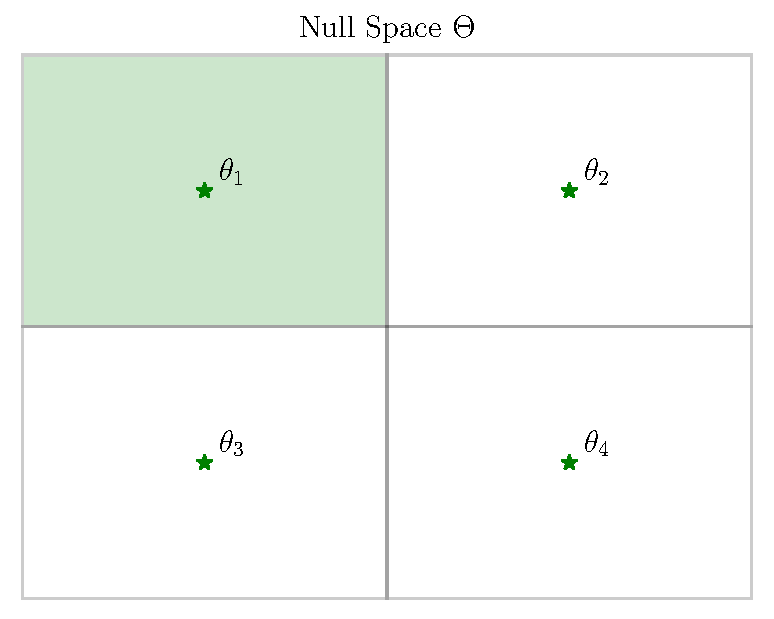
\includegraphics[width=0.95\linewidth]{figs/approach_4.pdf}
\end{figure} 
\end{frame}

\begin{frame}{Divide-and-Conquer for Guarantees on All of $\Theta$}
\begin{figure}
    \centering
    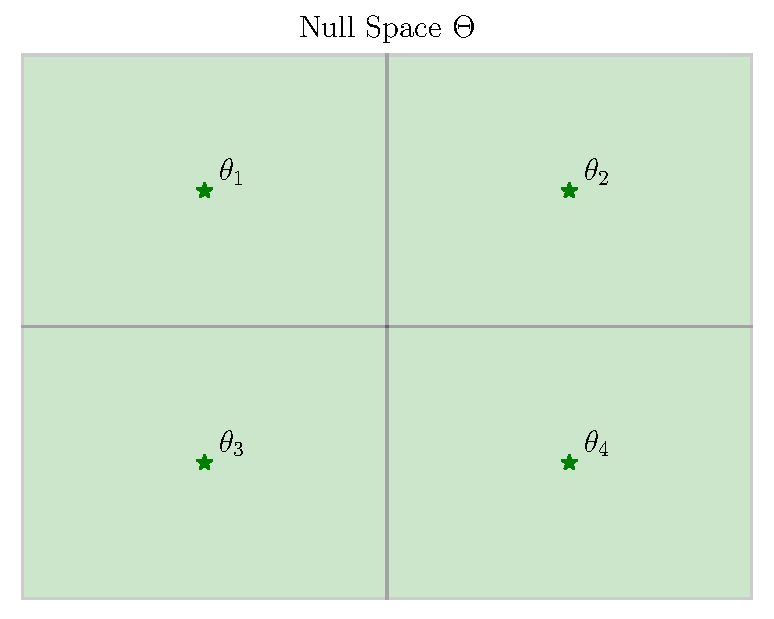
\includegraphics[width=0.95\linewidth]{figs/approach_5.pdf}
\end{figure} 
\end{frame}

\begin{frame}{Our Approach: Proof-by-Simulation}
\textbf{General Workflow:}
\begin{itemize}
    \item Let $\Theta$ be a (bounded) null hypothesis space.
    \item Partition $\Theta$ into tiles $\set{\Theta_i}_{i=1}^I$ 
        with representatives $\set{\theta_i}_{i=1}^I$.
    \item Simulate the design on each $\theta_i$ and output test statistics.
    \item Use our method \textbf{Continuous Simulation Extension} (CSE) to 
        \emph{extend} information at each $\theta_i$ to any other point in $\Theta_i$.
    \item Divide-and-conquer to get guarantees on \emph{all of $\Theta$}.
\end{itemize}
\end{frame}

\begin{frame}{Method 1: Validation for Point-wise Confidence}
\begin{figure}
    \centering
    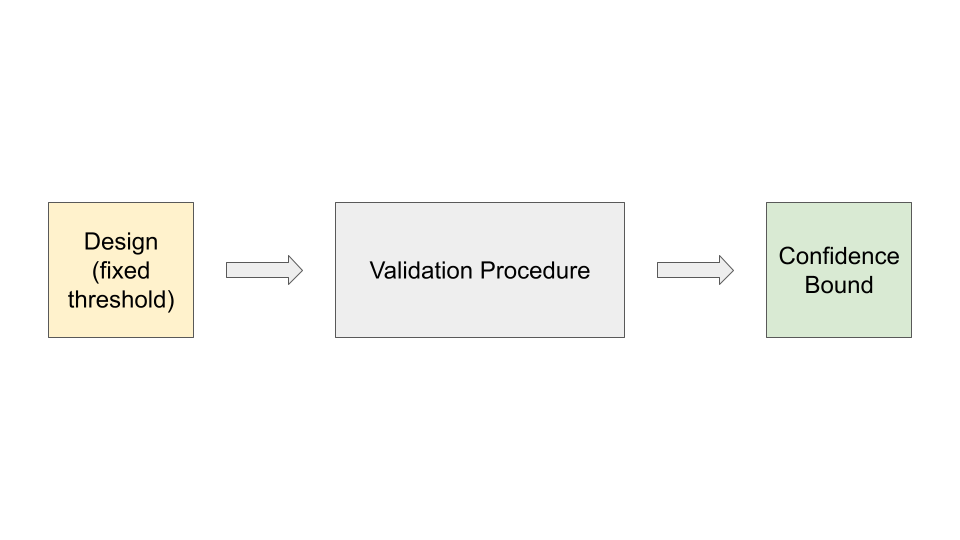
\includegraphics[width=\linewidth]{figs/validation_scheme.png}
\end{figure}
\end{frame}

\begin{frame}{Method 1: Validation for Point-wise Confidence}
\begin{itemize}
    \item \textbf{Validation}: 
        Construct bounds $(\hat{l}(\cdot), \hat{u}(\cdot))$
        for the true Type I Error, $f(\cdot)$, with confidence $1-\delta$:
        \begin{align*}
            \forall \theta \in \Theta ,\, 
            &\prob\pr{\hat{l}(\theta) \leq f(\theta)} \geq 1-\delta \text{ and } \\
            &\prob\pr{\hat{u}(\theta) \geq f(\theta)} \geq 1-\delta
        \end{align*}
    \item Point-wise guarantee is appropriate since 
        there is only one \emph{true} value of $\theta$.
\end{itemize} 
\end{frame}

\begin{frame}{Method 2: Calibration for Type I Error Proof}
\begin{figure}
    \centering
    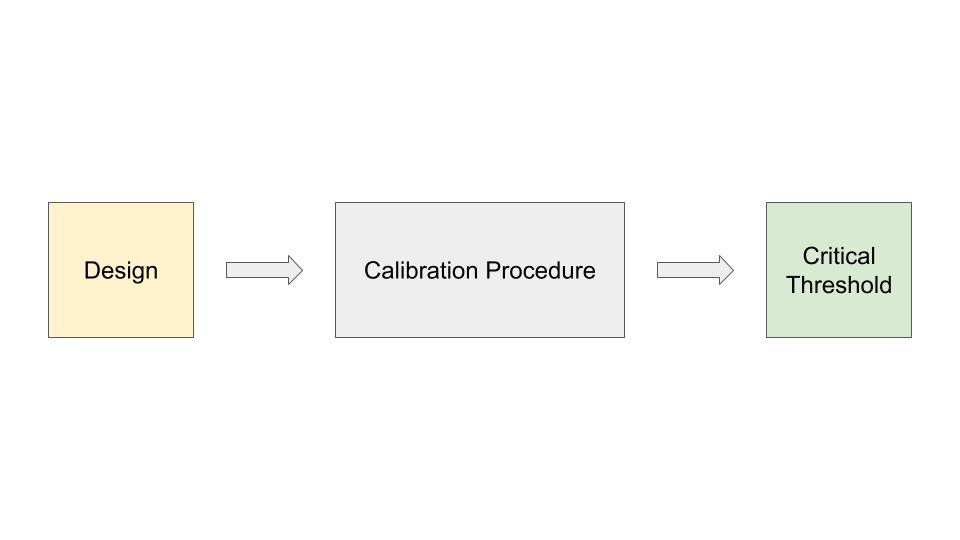
\includegraphics[width=\linewidth]{figs/calibration_scheme.png}
\end{figure}
\end{frame}

\begin{frame}{Method 2: Calibration for Type I Error Proof}
\begin{itemize}
    \item \textbf{Calibration}: 
        Select a (random) critical threshold, $\hat{\lambda}^*$, such that 
        \begin{align*}
        \forall \theta \in \Theta,\, 
        \EEE\br{f_{\hat{\lambda}^*}(\theta)} 
        \leq 
        \alpha
        \end{align*}
        where $f_{\lambda}(\theta)$ is the Type I Error at $\theta$
        using threshold $\lambda$.
\end{itemize} 
\end{frame}

\begin{frame}{Random $\hat{\lambda}^*$ is acceptable}
\begin{itemize}
    \item Guarantee is \textbf{overall} valid (regulators want this!).
    \item Practitioners \textbf{already use} simulations to evaluate designs.
    \item Our approach is \textbf{strictly stronger} because we can give guarantees.
\end{itemize}
\end{frame}
